\section{Numerical solver: Craig--Sulem expansion and Gauss--Legendre integration}
\label{sec:solver}

\subsection{Reference Dirichlet--Neumann operator}

For a horizontal bed and a free surface sufficiently close to the flat
state, the DNO is analytic in the surface elevation and admits the
Craig--Sulem expansion \cite{craig1993,xu2009}:
\begin{equation}
  \G(\eta;h)=\sum_{m=0}^{\infty}\G_m(\eta;h),
  \qquad \G_m(\lambda\eta;h)=\lambda^m\G_m(\eta;h).
  \label{eq:cs-expansion}
\end{equation}
Writing $D=-i\partial_x$, the first two terms are
\begin{align}
  \G_0(h)&=|D|\tanh(h|D|), \label{eq:g0}\\
  \G_1(\eta;h)\xi
  &=-\G_0(h)\bigl(\eta\G_0(h)\xi\bigr)
    -\partial_x\bigl(\eta\partial_x\xi\bigr).
  \label{eq:g1}
\end{align}
The historical rollout-derived labels and truth trajectories, as well as
every target in the forward dataset design, use the recursion through order
\(M=6\).
Products inside this expansion are computed by zero-padding Fourier
coefficients by a factor of eight, multiplying on the enlarged physical grid,
and truncating back to the base grid. Forward-dataset targets are projected
onto \(|k|\leq128\) and have zero mean. As documented in
\cref{sec:data}, three historical static sources retain unprojected stored
labels and are not retroactively described by the forward target convention.
These numerical choices are conservative because the order-\(M\) recursion
contains powers of the differentiation multiplier and can magnify unresolved
high-frequency roundoff as $|k|^M$.

The nonlinear expression in \eqref{eq:zakharov-xi} is also dealiased. Given
$q=\G(\eta;h)\xi$, we evaluate
\begin{equation}
  \mathcal N_\xi(\eta,\xi,q)
  =-\frac12\xi_x^2+
   \frac12\frac{(q+\eta_x\xi_x)^2}{1+\eta_x^2}
  \label{eq:xi-nonlinearity}
\end{equation}
on a grid with $2N$ points and then spectrally truncate to $N$ points. This
implements the equations-of-motion dealiasing advocated by Xu and Guyenne
\cite{xu2009}. Our diagnostics show that dealiasing removes a terminal
amplifier but does not by itself cure a learned-operator instability: for
failing states it delays the first nonfinite value only slightly because the
spectral cascade is already established before aliasing becomes large.

\subsection{Integrating-factor splitting}

We separate the exactly solvable linear gravity-wave system from its nonlinear
remainder. With \(u=(\eta,\xi)\), define
\begin{equation}
  \mathcal N(u)
  =
  \begin{bmatrix}
    \bigl(\G(\eta;h)-\G_0(h)\bigr)\xi\\
    \mathcal N_\xi(\eta,\xi,\G(\eta;h)\xi)
  \end{bmatrix}.
  \label{eq:nonlinear-remainder}
\end{equation}
In Fourier space, for each nonzero mode,
\begin{equation}
  \frac{\dd}{\dd t}
  \begin{bmatrix}\widehat\eta_k\\ \widehat\xi_k\end{bmatrix}
  =L_k
  \begin{bmatrix}\widehat\eta_k\\ \widehat\xi_k\end{bmatrix}
  +\widehat{\mathcal N}_k,
  \qquad
  L_k=\begin{bmatrix}0&g_0(k;h)\\-g&0\end{bmatrix},
  \quad g_0(k;h)=|k|\tanh(h|k|).
  \label{eq:linear-split}
\end{equation}
Since $L_k^2=-\omega_k^2I$ with
$\omega_k^2=gg_0(k;h)$ and \(I\) the \(2\times2\) identity, the matrix
exponential is available exactly for any time increment \(\tau\):
\begin{equation}
  e^{\tau L_k}=I\cos(\omega_k\tau)
  +\frac{L_k}{\omega_k}\sin(\omega_k\tau).
\end{equation}
With $v(t)=e^{-tL}u(t)$, the transformed equation is
\begin{equation}
  v_t=F(t,v):=e^{-tL}\mathcal N(e^{tL}v).
  \label{eq:if-system}
\end{equation}
This removes the stiff linear oscillation from the nonlinear stage equations
and gives exact linear dispersion independently of the step size.

\subsection{Two-stage Gauss--Legendre method}

We apply the two-stage Gauss--Legendre Runge--Kutta method to
\eqref{eq:if-system}. It is fourth-order accurate and symplectic for a
Hamiltonian vector field. Its Butcher coefficients are
\begin{equation}
  c_{1,2}=\frac12\mp\frac{\sqrt3}{6},\qquad
  A=\begin{bmatrix}
  \frac14&\frac14-\frac{\sqrt3}{6}\\[2pt]
  \frac14+\frac{\sqrt3}{6}&\frac14
  \end{bmatrix},\qquad b_1=b_2=\frac12.
  \label{eq:gl2-tableau}
\end{equation}
For a step from $t_n$ to $t_{n+1}=t_n+\Delta t$, with
\(v_n\approx v(t_n)\) and \(a_{ij}\) the entries of \(A\), the stages solve
\begin{align}
  Y_1&=v_n+\Delta t\left(a_{11}F(t_n+c_1\Delta t,Y_1)
                  +a_{12}F(t_n+c_2\Delta t,Y_2)\right),\\
  Y_2&=v_n+\Delta t\left(a_{21}F(t_n+c_1\Delta t,Y_1)
                  +a_{22}F(t_n+c_2\Delta t,Y_2)\right),
  \label{eq:gl2-stages}
\end{align}
Define $F_i=F(t_n+c_i\Delta t,Y_i)$ for $i=1,2$. The update is
\begin{equation}
  v_{n+1}=v_n+\frac{\Delta t}{2}\left(F_1+F_2\right).
  \label{eq:gl2-update}
\end{equation}
The historical v9 trajectories and the forward Tanaka and Benjamin--Feir
contracts use at most four simultaneous Picard updates for
\eqref{eq:gl2-stages}.  The forward JONSWAP/TMA contract uses at most five;
this extra update was fixed together with its larger internal grid and does
not change the convergence test.  The forward dataset declares a stage
converged only when
\begin{equation}
  \max_{\substack{i\in\{1,2\}\\z\in\{\eta,\xi\}}}
  \frac{\|\Phi_i^z-Y_i^z\|_{\ell^2}}
       {\max\{\|\Phi_i^z\|_{\ell^2},
              \|Y_i^z\|_{\ell^2},
              \operatorname{tiny}\}}
  \leq10^{-8},
  \label{eq:gl2-stage-residual}
\end{equation}
where \(\Phi_i\) is the right-hand side of the \(i\)-th stage equation and
\(\operatorname{tiny}\) is the smallest positive normal float64 number. The
superscript \(z\in\{\eta,\xi\}\) labels the two component arrays, and
\(\|\cdot\|_{\ell^2}\) is their discrete norm. The implementation evaluates
this norm on Fourier coefficients; Parseval's identity gives the same ratios
as the physical-grid norm. Step sizes and output cadences are specified with
their corresponding dataset protocols in \cref{sec:data}. The nonlinear
right-hand side is projected after its dealiased evaluation; after each
accepted step, both state fields are projected to the same resolved subspace
and the mean of \(\xi\) is set to zero.

Symplecticity alone does not protect a surrogate rollout. It applies to the
Hamiltonian vector field actually supplied to the method. If
$\eta_t=\Gtheta(\eta;h)\xi$ is combined with a $\xi_t$ that is not the variation
of the same learned kinetic energy, then the vector field is noncanonical and
the usual Hamiltonian-structure argument for Gauss--Legendre integration no
longer applies. Moreover, once the learned tangent gain becomes sufficiently
large, the Picard map in
\eqref{eq:gl2-stages} ceases to be contractive. In our failure traces this is
the terminal event, not the initial source of the error.

\subsection{Soliton-selective spectral-envelope guard}
\label{sec:soliton-guard}

The structured operator removes nonfinite rollouts, but one close two-soliton
interaction still develops a resolved spectral cascade. We introduce a
conditional stabilization for this failure mode. It is deliberately distinct
from the fixed projection used by the reference solver: the guard is exactly
inactive whenever the profile-based test below fails, and is nearly the
identity on a trajectory for which it is active until the initially empty
production band grows abnormally.

First, the initial condition is classified using only its surface profile. Let
\begin{equation}
  r_-(\eta_0)
  =\frac{\norm{\min(\eta_0,0)}_2^2}{\norm{\eta_0}_2^2}.
  \label{eq:negative-energy-selector}
\end{equation}
Here the minimum is taken pointwise and \(\|\cdot\|_2\) is the discrete
spatial norm.
The guard is active only when
\begin{equation}
  s_0
  =\mathbf 1\!\left\{r_-(\eta_0)<10^{-3}\right\}
   \mathbf 1\!\left\{\operatorname{mean}(\eta_0)>0\right\}=1.
  \label{eq:soliton-selector}
\end{equation}
Here \(\operatorname{mean}(\eta_0)=N^{-1}\sum_{j=0}^{N-1}\eta_0(x_j)\).
This is a profile-based activation test, not a wave-family label. In the
evaluation dataset all 64 Tanaka initial conditions satisfy
$r_-\leq2.11\times10^{-4}$, whereas the minimum over the inspected
non-Tanaka conditions is $0.257$.

\begin{figure}[t]
  \centering
  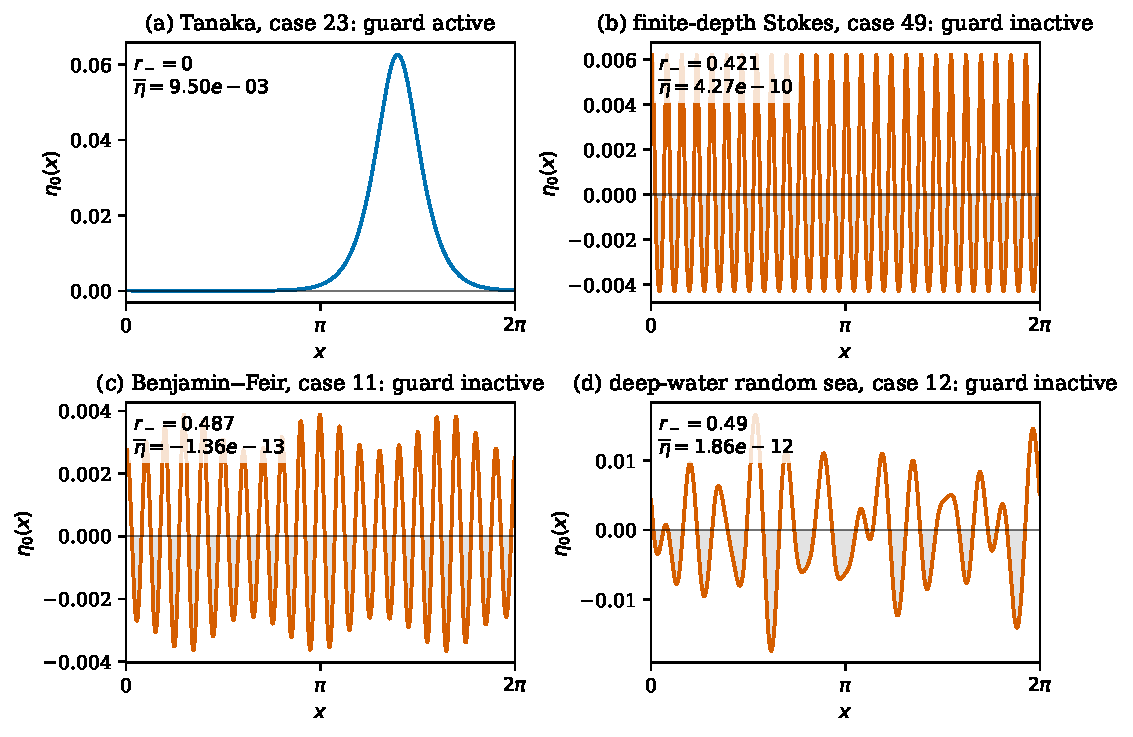
\includegraphics[width=0.96\linewidth]{figures/soliton_selector_examples.pdf}
  \caption{Examples of the initial-condition selector in
  \eqref{eq:soliton-selector}.  Gray shading marks the negative part of each
  surface profile.  The Tanaka profile has negative-energy fraction below
  $10^{-3}$ and positive mean, so the guard is active.  For the three
  non-Tanaka profiles the negative-energy fraction
  exceeds the threshold, so the guard is inactive.  All four cases remain in
  the rollout evaluation.}
  \label{fig:soliton-selector-examples}
\end{figure}

The selector does not estimate oscillation, localization, or family identity.
It tests only the negative-energy fraction and the mean in
\eqref{eq:soliton-selector}; the examples in
\cref{fig:soliton-selector-examples} illustrate the resulting guard state.

For the unnormalized discrete Fourier transform $\widehat\eta_k$, define the
production-band amplitude
\begin{equation}
  A(t)=\frac{1}{N}
  \left(\frac{1}{N}\sum_k
  \mathbf 1_{\{64\leq |k|<128\}}|\widehat\eta_k(t)|^2\right)^{1/2},
  \qquad
  A_{\mathrm{tr}}=\max\!\left(5\times10^{-7},100A(0)\right).
  \label{eq:guard-amplitude}
\end{equation}
The transition is smoothed in logarithmic amplitude,
\begin{equation}
  w(t)=s_0
  \left[1+\exp\!\left(-10\log\frac{A(t)}{A_{\mathrm{tr}}}\right)\right]^{-1}.
  \label{eq:guard-weight}
\end{equation}
We set \(w(t)=0\) when \(A(t)=0\). Thus $w=1/2$ at the threshold, while
$w\approx10^{-10}$ when
$A/A_{\mathrm{tr}}=0.1$. This avoids a discontinuous switch in the numerical
flow.

Once the envelope grows, both canonical variables are multiplied after each
Gauss--Legendre substep by a blended eighth-order Hou--Li-type filter
\cite{hou2007},
\begin{align}
  \sigma_h(k)
  &=\exp\!\left[-0.69
    \left(\frac{|k|}{k_{\mathrm{eff}}(h)}\right)^8\right],
  &k_{\mathrm{eff}}(h)&=\min\!\left(128,\frac{12}{h}\right),
  \label{eq:depth-houli}\\
  \widehat u_k^{\,+}
  &=\left[(1-w)+w\sigma_h(k)\right]\widehat u_k^{\,-},
  &u&\in\{\eta,\xi\}.
  \label{eq:guard-update}
\end{align}
The scale $k_{\mathrm{eff}}h\leq12$ follows the depth scaling of a solitary
wave's horizontal width. It is conservative relative to the truth-spectrum
audit: across the 64 Tanaka reference rollouts, removing content with
$|k|h>8$ changes $\eta$ and $\xi$ by at most
$1.22\times10^{-9}$ and $2.94\times10^{-11}$, respectively, at the 99th
percentile. For the failing depth $h=0.17760$,
$k_{\mathrm{eff}}=67.57$; for the shallow phase-error case,
$12/h>128$, so no additional depth restriction is introduced. The guard is
therefore a conditional spectral viscosity, not a hard global cutoff.
